\subsection{Overview of Installation} \label{subsection:android-install}
%START TEXT INPUT

Installation two steps:  primary is the APK verification and secondary is the bytecode optimization/art\newline
legitimate signature as well as correct classes.dex structure cannot be verified are rejected for installation by the OS\newline
Once verified, the .dex file is forwarded for optimization: a necessary step due to the high diversity of Android running hardware (dex)-see- Dalvik executable is a generic file format which needs additional processing to achieve best performance for the concrete device architecture (odex)\newline
optimization\newline
step removes the classes.dex from the original APK archive and loads in memory the .odex file upon execution, occurs only once, during the initial run of the application which explains the usually slower first application launch comparing to the subsequent ones\cite{kovachevaMaster}
\begin{figure}[h]
    \centering
    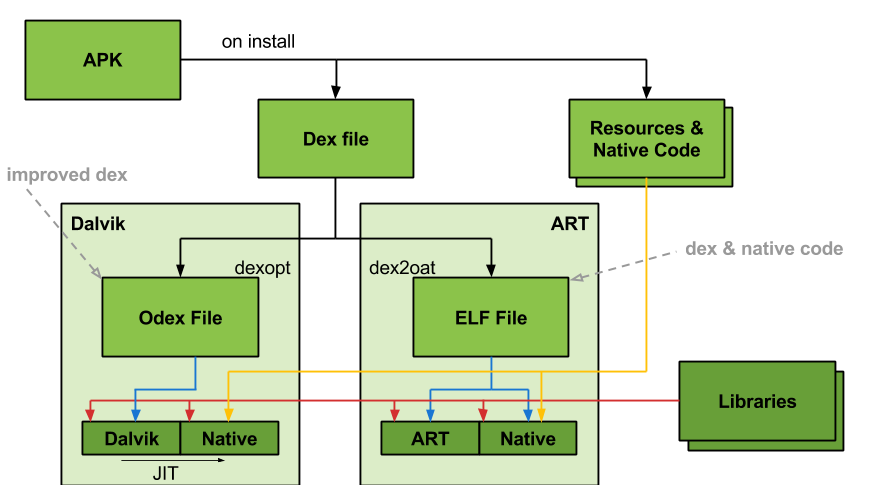
\includegraphics[width=0.8\textwidth]{data/install.png}
    \caption{install}
    \label{fig:install}
\end{figure}

In order to create a sandboxed environment, Android assigns each application a seperate user ID on install to ensure that nobody except users with the same ID can access the applications resources.
The Android operating system is a multi-user Linux system in which each app is a different user.
By default, the system assigns each app a unique Linux user ID (the ID is used only by the system and is unknown to the app). The system sets permissions for all the files in an app so that only the user ID assigned to that app can access them
Each process has its own virtual machine (VM), so an app's code runs in isolation from other apps.
By default, every app runs in its own Linux process. Android starts the process when any of the app's components need to be executed, then shuts down the process when it's no longer needed or when the system must recover memory for other apps\cite{developerFundamentals}

%START TEXT INPUT

%
%Installation two steps:  primary is the APK verification and secondary is the bytecode optimization/art\newline
%legitimate signature as well as correct classes.dex structure cannot be verified are rejected for installation by the OS\newline
%Once verified, the .dex file is forwarded for optimization: a necessary step due to the high diversity of Android running hardware (dex)-see- Dalvik executable is a generic file format which needs additional processing to achieve best performance for the concrete device architecture (odex)\newline
%optimization\newline
%step removes the classes.dex from the original APK archive and loads in memory the .odex file upon execution, occurs only once, during the initial run of the application which explains the usually slower first application launch comparing to the subsequent ones

%ablauf starten von app\newline
%When an Android application is executed, the process consists of the following four parts:
%• Dalvik bytecode, which is located in the dex file
%• Dalvik Virtual Machine [13], which executes the Dalvik bytecode
%• Native Code, like shared objects, which is executed by the processor
%• Android Application Framework, which provides services for the application\newline
%\cite{kovachevaMaster}
%




%
%The Android operating system is a multi-user Linux system in which each app is a different user.
%By default, the system assigns each app a unique Linux user ID (the ID is used only by the system and is unknown to the app). The system sets permissions for all the files in an app so that only the user ID assigned to that app can access them
%Each process has its own virtual machine (VM), so an app's code runs in isolation from other apps.
%By default, every app runs in its own Linux process. Android starts the process when any of the app's components need to be executed, then shuts down the process when it's no longer needed or when the system must recover memory for other apps

%\cite{developerFundamentals}
%
